%%%%%%%%%%%%%%%%%%%%%%% file template.tex %%%%%%%%%%%%%%%%%%%%%%%%%
%
% This is a general template file for the LaTeX package SVJour3
% for Springer journals.          Springer Heidelberg 2010/09/16
%
% Copy it to a new file with a new name and use it as the basis
% for your article. Delete % signs as needed.
%
% This template includes a few options for different layouts and
% content for various journals. Please consult a previous issue of
% your journal as needed.
%
%%%%%%%%%%%%%%%%%%%%%%%%%%%%%%%%%%%%%%%%%%%%%%%%%%%%%%%%%%%%%%%%%%%
%
% First comes an example EPS file -- just ignore it and
% proceed on the \documentclass line
% your LaTeX will extract the file if required
\begin{filecontents*}{example.eps}
%!PS-Adobe-3.0 EPSF-3.0
%%BoundingBox: 19 19 221 221
%%CreationDate: Mon Sep 29 1997
%%Creator: programmed by hand (JK)
%%EndComments
gsave
newpath
  20 20 moveto
  20 220 lineto
  220 220 lineto
  220 20 lineto
closepath
2 setlinewidth
gsave
  .4 setgray fill
grestore
stroke
grestore
\end{filecontents*}
%
\RequirePackage{fix-cm}
%
%\documentclass{svjour3}                     % onecolumn (standard format)
%\documentclass[smallcondensed]{svjour3}     % onecolumn (ditto)
\documentclass[smallextended]{svjour3}       % onecolumn (second format)
%\documentclass[twocolumn]{svjour3}          % twocolumn
%
\smartqed  % flush right qed marks, e.g. at end of proof
%
\usepackage{graphicx}
\usepackage{hyperref}
\usepackage{varioref}
\usepackage{url}
\usepackage{epsfig}
\usepackage{amsmath}
\usepackage{epsfig}
\usepackage{amssymb}
\usepackage{graphicx}
\usepackage{algorithm2e}
\usepackage{algorithmic}
\usepackage{subfigure}
%
% \usepackage{mathptmx}      % use Times fonts if available on your TeX system
%
% insert here the call for the packages your document requires
%\usepackage{latexsym}
% etc.
%
% please place your own definitions here and don't use \def but
% \newcommand{}{}
%
% Insert the name of "your journal" with
% \journalname{myjournal}
%
\newcommand{\fix}{\marginpar{FIX}}
\newcommand{\new}{\marginpar{NEW}}
\newtheorem{defn}{Definition}
\newtheorem{thm}{Theorem}
%\newcommand{\theoremname}{Assumption}
\newcounter{asm}
\newenvironment{asm}{%
  \par\medskip\refstepcounter{asm}%
  \noindent\textbf{Assumption \theasm:}\quad}{\par\medskip}
\labelformat{asm}{\theoremname~#1}

\begin{document}

\title{Consensus-Based Large-Scale Selection of Features%\thanks{Grants or other notes
%about the article that should go on the front page should be
%placed here. General acknowledgments should be placed at the end of the article.}
}
\subtitle{}

%\titlerunning{Short form of title}        % if too long for running head

\author{Haimonti Dutta        \and
        Ashwin Srinivasan %etc.
}

%\authorrunning{Short form of author list} % if too long for running head

\institute{Haimonti Dutta \at
            The Center for Computational Learning Systems (CCLS)  \\
            Columbia University\\
			New York, NY 10115. \\
			\email{haimonti@ccls.columbia.edu} \\
                  %  \\
%             \emph{Present address:} of F. Author  %  if needed
           \and
           Ashwin Srinivasan \at
		   Department of Computer Science \\
		   IIIT, Delhi.\\
		   \email{ashwin@iiitd.ac.in}\\
}

\date{Received: date / Accepted: date}
% The correct dates will be entered by the editor


\maketitle

\begin{abstract}
Insert your abstract here. Include keywords, PACS and mathematical
subject classification numbers as needed.
\keywords{First keyword \and Second keyword \and More}
% \PACS{PACS code1 \and PACS code2 \and more}
% \subclass{MSC code1 \and MSC code2 \and more}
\end{abstract}

\section{Introduction}
\label{intro}

The field of Inductive Logic Programming (ILP) has made steady
progress over the past two decades, in advancing the theory,
implementation and application of logic-based relational learning \cite{something}.
A characteristic of this form of machine-learning is that
data, prior knowledge and hypotheses are usually---but not always---expressed in a
subset of first-order logic, namely logic programs.
Side-stepping for the moment the question ``why logic programs?'', it is evident
that settling on some variant of first-order logic allows the construction of tools that
enable the automatic construction of descriptions that use relations
(used here in the formal sense of a truth value assignment to $n$-tuples).
There are at least two kinds of 
tasks where some form of relational learning would appear to be necessary:

\begin{enumerate}
    \item[(a)] The construction of models of systems
    that explicitly require relations. Examples are graphical models,
        grammars, recursive definitions, and so on.
    \item[(b)] The identification of functions
        (again used formally, in the sense of being a uniquely
        defined relation) whose domain is the set of instances in the data.
        An example is the construction of new ``features'' for data analysis
        based on existing relations (``$f(m) = y$ if a molecule $m$ has 3 or more
        benzene rings fused together otherwise $f(m) = n$''). 
\end{enumerate}

\noindent
Feature-construction in (b) would seem to be no more
than just a special form of relation-learning as decribed in (a) above. In
principle, this is correct. However, the
features are not intended to constitute a stand-alone
description of a system's structure. Instead, their purpose is to enable
different kinds of data analysis to be performed better. These may be constructing models
for discrimination, joint probability distributions,
forecasting, clustering, and so on. If a logic-based relational learner like an ILP
engine is used to construct these relational features,
then each feature is formulated as a logical formula.
A measure of comprehensibility will be retained in the resulting models that use
these features (see Fig. ~\ref{fig:features}).

\begin{figure}[h]
\centerline{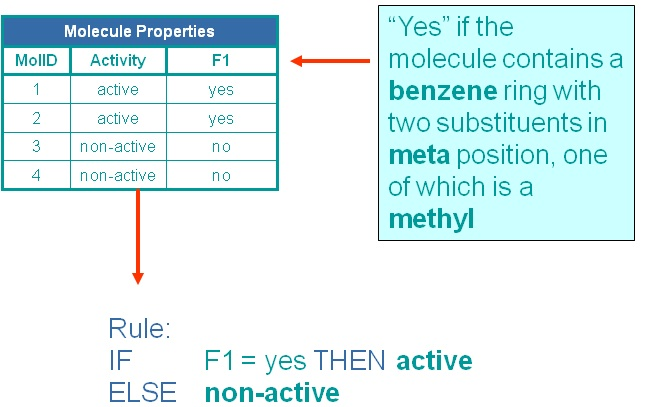
\includegraphics[height=4cm]{features.jpg}}
\caption{Feature discovery with relational learning. If we knew feature
F1, it is easy to construct a model for active molecules using any
machine learning program (rule at the bottom).
What we are talking about here is discovering the definition of F1 (box on
the right), given relational descriptions of the molecules
m1--m4. Once done, we may be able to construct better
models for the data.}
\label{fig:features}
\end{figure}

The approach usually, but not always, separates relational learning
(to discover features) and modelling
(to build models using these features). There will of course
be problems that require the joint identification of relational
 with features and models---the emerging area of statistical relational
learning (SRL), for example, deals with the conceptual and implementation issues
that arise in the joint estimation of statistical parameters and relational
models. It would appear that separate construction of features
and statistical models would represent no more than a poor man's SRL.
Nevertheless, there is now a growing body of
research that suggests that augmenting any existing
features with ILP-constructed relational ones can substantially
improve the predictive power of a statistical model \cite{something}.
There are thus  very good practical reasons to persist with this variant of
statistical and logical learning for data analysis.

There are however shortcomings with the approach which limit its
applicability to large-scale problems. First, the set possible relational features
is usually not finite This has led to an emphasis on syntactic and
semantic restrictions constraining the features to some finite set. In practice
this set is still very large, and it is intractable to identify an optimal
subset of features. ILP engines for feature-construction therefore employ some form
of heuristic search, with no specific guarantees associated with the result.
Second, much still needs to be done to scale ILP-based feature discovery
up to meet modern data and model requirements. This includes the abilities to
discover features using very large datasets not all stored in one place,
and only in secondary memory; from relational data arriving in a streaming mannery;
and from data which do not conform easily to expected patterns.

This paper addresses some of these limitations: not in full measure, but for a class
of models and loss-function. Specifically, we describe how a network of computational
nodes can be used to construct optimal (or near-optimal) linear models for discrimination.
Each node has access to some (but not all) relational features constructed by an ILP
engine. Using a simple consensus-based algorithm, all nodes in the network converge on
the optimal weights for all the features. The setting is naturally amenable to
parallelisation, and empirical results obtained using the approach are encouraging.
The rest of the paper is organised as follows. Section \ref{sec:example}
shows an example of what we expect to achieve, using a simple synthetic
dataset. Section \ref{sec:ilp} is a short
introduction to ILP and its use in constructing features. Section \ref{sec:probdesc}
formulates the problem as one of consensus-based model construction. Section \ref{sec:alg}
presents an iterative procedure for constructing models in a network of nodes capable
of exchanging information about their local models. The section includes a proof of
convergence and termination for linear models. The algorithm is evaluated empirically
on a number of standard ILP benchmarks in Section \ref{sec:expt}. Section
\ref{sec:work} describes related work and open issues. Section \ref{sec:concl}
concludes the paper.

\section{Consensus-based Feature Selection for ILP Applications}
\label{sec:example}

\begin{figure}[h]
\centerline{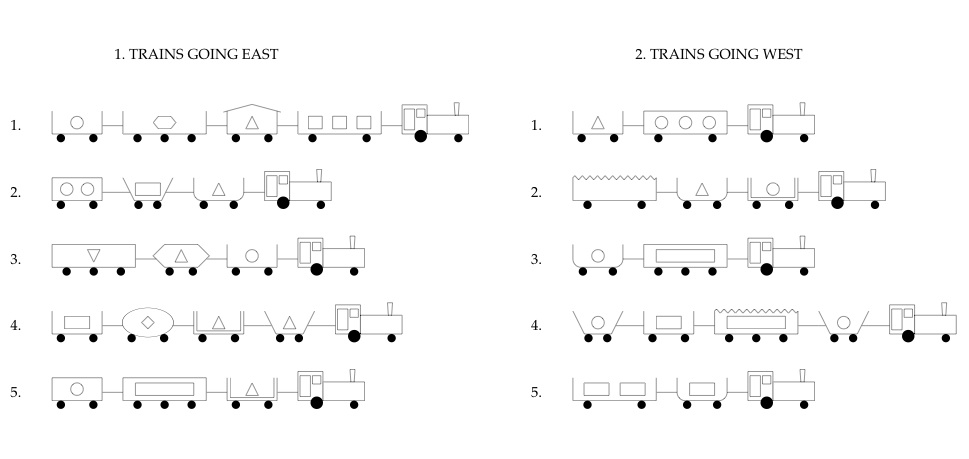
\includegraphics[width=1\textwidth,height=0.32\textheight ]{trains.jpg}}
\caption{The train spotting dataset. There are two sets of trains: Eastbound and Westbound. Descriptors for the trains include: number, shape and lengths of the car, shape of load, and so on. The task is to determine decision rules to distinguish between them. }
\label{trains}
\end{figure} 

\noindent We motivate the task of consensus-based feature selection using the train spotting problem, originally proposed by Ryzhard Michalski \cite{Larson_77}. Given two sets of trains: eastbound and westbound, the problem is to determine decision rules to distinguish between train sets, using properties of the carriages and load carried (Figure~\ref{trains}). For example, a decision rule can be: 
 \begin{align} 
 \nonumber &[NCARS=4] \\ 
  \nonumber &[IF (CAR_1, CAR_2)][INFRONT(CAR_2,CAR_3)][INFRONT(CAR_3,CAR_4)] \\
 \nonumber
 &[CAR-SHAPE(CAR_1)=ENGINE] [CAR-SHAPE(CAR_2)=U-SHAPED] \\
 \nonumber &[CAR-SHAPE(CAR_3)=OPEN-TRAPEZOID] \\
 \nonumber &[CAR-SHAPE(CAR_4)=RECTANGLE][LN(CAR_1)=LONG] \\
 \nonumber &[LN(CAR_2)=SHORT][LN(CAR_3)=SHORT][LN(CAR_4)=SHORT] \Rightarrow [D=EAST].
\end{align}
where the features are: (1) $NCARS$: number of cars, (2) $CAR-SHAPE(car)$: shape of a car, (3) $LN(car_i)$:length of a car, (4)$INFRONT(car_i,car_j)$: predicate indicating that $car_i$ is infront of $car_j$.

We assume that trains can be adequately described by background predicates and that $10$ trains shown in the figure are denoted by $t1, t2, \cdots, t10$. The classification of trains can be encoded by logical statements of the form $Class(t1,eastbound),Class(t2,eastbound) \cdots, Class(t10,westbound)$. All features are assumed to be boolean valued as is common in ILP applications \cite{Specia_09}.

Suppose $500$ such features are randomly generated by an ILP engine for the train spotting problem. Our task is to find the subset of features that result in the best model. An exhaustive search in the space of $2^{500}$ features is clearly intractable. Are we, however, able to partition the feature space, such that compute nodes in a distributed environment could individually work with subsets, \emph{gossip} with neighboring nodes to exchange information and eventually agree on a set of \emph{consensus} features? The algorithm for distributed feature estimation, described in Section~\ref{sec:probdesc}, takes a step in that direction.

\section{Related Work}
\label{sec:related}

\noindent \textbf{ILP Applications }Existing literature on discovering a subset of discriminative features from inductive logic programming applications can be classified as follows: strategies that pose the problem as a (a)discrete optimization problem that is solved optimally~\cite{l1Reg,cvpr2007,nips2004} or heuristically~\cite{JoshiRS08,Amrita12,NageshRCKDB12,ChalamallaNSR08,SpeciaSJRN09,RamakrishnanJBS07,SpeciaSRN06} (b) convex optimization problem with sparsity inducing regularizers that solves it optimally~\cite{JawanpuriaNR11,NairSRK12} (c) computes all relational features that satisfy some quality criterion by systematically and efficiently exploring a prescribed search space~\cite{pei2004,subseqGap2006,bitSpade,antunes2003,han2005,rakesh1995,han2004,gehrke2002,rastogi1999}.

  
\noindent \textbf{Other Domains }
\section{Feature Discovery}
\label{sec:ilp}

\section{Problem Statement}
\label{sec:probdesc}
Let $M$ denote an $n \times m$ matrix with real-valued entries.  This matrix 
represents a dataset of $n$ tuples of the form $X_i \in \mathbb{R}^m, 1 \le i \le n$.  
%Let $M^j$ denote the $j^{th}$ column and $M^j(i)$ denote the $i^{th}$ entry of this column.  
%Let $\mu(M^j)$ denote the {\em sample mean} of this column, 
%$\frac{\sum_{i=1}^{n}M_j(i)}{n}$.  Let $Var(M^j)$ denote the 
%{\em sample variance} of this column, 
%$\frac{\sum_{i=1}^{n}[\mu(M^j) - M^j(i)]^2}{n-1}$.  
%%Let $Cov(M^j,M^k)$ denote the 
%{\em sample covariance} of the $j^{th}$ and $k^{th}$ columns,
%$\frac{\sum_{i=1}^{n}[\mu(M^j) - M^j(i)][\mu(M^k) - M^k(i)]}{n-1}$.
%Note, $Var(M^j)$ $=$ $Cov(M^j,M^j)$).  Finally, let $Cov(M)$ denote the 
%{\em covariance matrix} of $M$ {\em i.e.} the $m \times m$ matrix whose 
%$(j,k)^{th}$ entry is $Cov(M^j,M^k)$.  
Assume, without loss of generality, this dataset has been vertically distributed over $k$ sites $S_1, S_2, \cdots, S_k$ i.e. site $S_1$ has $m_1 $ attributes, $S_2$ has $m_2$ attributes and so on, such that $|m_1| + |m_2|+ \cdots + |m_k| = |m|$, where $|m_i|$ represents the number of attributes at site $S_i$\footnote{In the more general setting, Site $S_i$ has a random subset of features $m_i \subset m$.}. 
Let $M_1$ denote the $n \times m_1$ matrix representing the dataset held by $S_1$,
$M_2$ denote the $n \times m_2$ matrix representing the dataset held by $S_2$ and so on.
Thus, $M = M_1:M_2: \cdots : M_k$ denotes the concatenation of the local datasets. %The $j^{th}$ column of $A:B$ is denoted $[A:B]^j$.
%Assume this dataset has been vertically distributed over two sites $S_A$ and $S_B$ -- thus, $S_A$ 
%has the first $p$ attributes and $S_B$ has the last $q$ attributes ($p+q = m$).
%Let $A$ denote the $n \times p$ matrix representing the dataset held by $S_A$,
%and $B$ denote the $n \times q$ matrix representing the dataset held by $S_B$.
%Let $A:B$ denote the concatenation of the datasets {\em i.e.} $M = A:B$.
%The $j^{th}$ column of $A:B$ is denoted $[A:B]^j$.

%Following a standard practice in applied statistics, we pre-process $M$ by normalizing so that $\mu(M^j) = 0$ and $Var(M^j) = 1$.  This is achieved by replacing each entry 
%$M^j(i)$ with 
%$\frac{M^j(i) - \mu(M^j)}{\sqrt{Var(M^j)}}$.  Since both $\mu(M^j)$ and $Var(M^j)$
%can be computed without any communication, then normalizing can be performed without
%any communication.  Henceforth, we assume $\mu(M^j) = 0$ and $Var(M^j) = 1$.  

The goal is to learn a linear discriminative function over the data set $M$. The global function to be estimated is represented by $f_{g} = M W_{g}^{T} $ where $W_g$ is assumed to be a $1 \times m$ weight vector. If only the local data is used, at site $S_1$, the local function estimated would be $f_1 = M_1 W_{1}^{T}$. At site $S_2$, the local function estimated would be $f_2 = M_2 W_{2}^{T}$. The goal is to describe a de-centralized algorithm for computing the weight vectors at sites $S_1, \cdots S_k$ such that on termination $W_{1} \approx W_g[1:m_1], W_2 \approx W_g[1:m_2], \cdots W_k \approx W_g[1:m_k]$ where $W_g[1:m_i]$ represents the part of the global weight vector for the attributes stored at that site $S_i$. Clearly, if all the datasets are transferred to a central location, the global weight vector can be estimated. Our objective is to learn the function in the decentralized setting assuming that transfer of actual data tuples is expensive and may not be allowed (say for example due to privacy concerns). The weights obtained at each site on termination of the algorithm will be used for ranking the features. \\

%\noindent \textbf{An Example: } Let $S_A$ have $A = [X_1 X_2 X_3]$ and $S_B$ have $B=[X_4]$. Local functions are $f_A = [X_1 X_2 X_3] [W_{A}^1 W_{A}^2 W_{A}^3 ]^{T}$ and $f_B = [X_4] [W_{B}^1 ]^{T}$. Global function to be learnt: $f_g = [X_1 X_2 X_3 X_4] [W_{A}^1 W_{A}^2 W_{A}^3 W_B^{1} ]^{T}$. Site A needs to get $f_B$ or some approximation of it and site B needs to get some approximation of $f_A$. Once this is done, both sites A and B have an approximation of the global function $f_g$. Next, each site must independently compute the gradient using Stochastic Gradient Descent (SGD). 



\section{Distributed Feature Estimation Algorithm}
\label{sec:alg}

\subsection{Building Blocks: Distributed Scalar Product Computation}
\label{sec:dotProd}
Several distributed scalar product computation protocols have been studied in literature(\cite{Du_01a},\cite{Du_01b}, \cite{Vaidya_02}). The goal is to ensure that each node in the distributed environment has the scalar product of the local vectors of all other nodes (possibly securely, when privacy needs to be preserved). We introduce a two-party scalar product computation protocol that the Distributed Feature Estimation Algorithm (described in~\ref{alg:fs}) relies on.

\noindent \textbf{Problem 1: } Site $S_1$ has $n$ instances with features $X_1^i, \cdots, X_p^i$ and weight vectors $W_1^i, \cdots, W_p^i$. Site $S_2$ has $n$ instances with features $X_{p+1}^i, \cdots, X_m^i$ and weight vectors $W_{p+1}^i, \cdots W_m^i$ respectively. Site $S_1$ and $S_2$ need to obtain the scalar product $\sum_{i=1}^{m} X_i^j W_i^j, 1 \le j \le n$ for all the $n$ instances.  \\

Consider the following naive solution: Site $S_1$ sends features and weights for all its $n$ instances to Site $S_2$; Site $S_2$ then computes the required scalar product. Clearly, in this case the communication cost involved is large i.e. $O(n \times p)$ and all of the data tuples need to be exchanged. 

A better solution would be if Site $S_1$ sent only the local scalar product for all $n$ instances, i.e. $\sum_{i=1}^{p} X_i^j W_i^j, 1 \le j \le n$. The communication cost in this case would be $O(n)$. Site $S_2$ on receiving the scalar product from $S_1$ adds it to its own local estimate i.e. $\sum_{i=1}^{p} X_i^j W_i^j +\sum_{i=1}^{m-(p+1)} X_i^j W_i^j  , 1 \le j \le n$. Site $S_2$ has effectively computed $\sum_{i=1}^{m} X_i^j W_i^j, 1 \le j \le n$ for all the $n$ instances. This additive nature of the protocol makes it amenable for use in distributed settings. 

\subsection{Assumptions}
\label{assum}

We state the following assumptions under which the Distributed Feature Estimation algorithm operates: \\

\noindent \textbf{Model of Distributed Computation} The distributed algorithm evolves over discrete time with respect to a ``global" clock\footnote{Existence of this clock is of interest only for theoretical analysis.}. Each site has access to a local clock or no clock at all. Furthermore, each site has its own memory and can perform local computation (such as computing the gradient on its local attributes). It stores $f_i$, which is the estimated local function. Besides its own computation, sites may receive messages from their neighbors which will help in evaluation of the next estimate for the local function.\\

\noindent \textbf{Communication Protocols} Sites $S_i$ are connected to one another via an underlying communication framework represented by a graph $G (V, E)$, such that each site  $S_i \in \{S_1, S_2, \cdots , S_k\}$ is a vertex and an edge $e_{ij} \in E$ connects sites $S_i$ and $S_j$. Communication delays on the edges in the graph are assumed to be zero. It must be noted that the communication framework is usually expected to be application dependent. In cases where no intuitive framework exists, it may be possible to simply rely on the physical connectivity of the machines, for example, if the sites $S_i$ are part of a large cluster. \\

\subsection{Algorithm Description}
\label{algo}

\noindent Algorithm~\ref{alg:fs} describes how the weights for attributes will be estimated using a consensus-based protocol. There are two main sub-parts of the algorithm: (1) Exchange of local function estimate and (2) Local update based on stochastic gradient descent. Each of these sub-parts are discussed in further detail below.   Furthermore, assume that $J: R^m \rightarrow [0, \infty]$ is a continuously differentiable nonnegative cost function with a Lipschitz continuous derivative.\\

\begin{algorithm}[t]
\small
{
\SetKwData{Left}{left}\SetKwData{This}{this}\SetKwData{Up}{up}
\SetKwFunction{Union}{Union}\SetKwFunction{FindCompress}{FindCompress}
\SetKwInOut{Input}{input}\SetKwInOut{Output}{output}

%\Input{$n \times m_i$ matrix at each site $S_i$; \\
%	   $G(V, E)$ which encapsulates the underlying communication framework; \\
%	   $T: $ no of iterations} 
\KwIn{$n \times m_i$ matrix at each site $S_i$, $G(V, E)$ which encapsulates the underlying communication framework, $T: $ no of iterations }
\KwOut{Each site $S_i$ has $W_i \approx W_g[1: m_i]$ }
%\Output{Each site $S_i$ has $W_i \approx W_g[1: m_i]$ }
\BlankLine

 %
 %\KwData{$n \times m_i$ matrix at each site $S_i$; Graph $G(V, E)$ which encapsulates the underlying communication framework; $T: $ no of iterations}
 %\KwResult{Each site $S_i$ has $W_i \approx W_g[1: m_i]$ }
 %initialization\;
\For{t = 1 to T}
 {
  (a) Site $S_i$ computes $M_i W_i^T$ locally and estimates the loss function\;
  (b) Site $S_i$ gossips with its neighbors $S_j \in \{N_i\}$ and obtains $M_j W_j^T$ for each neighbor\;
  (c) Site $S_i$ locally updates its function estimate as $J_i^t = \alpha_{ii}(M_i W_i^T) + \alpha_{ji} (M_j W_j^T)$ \;
  (d) Update the local weight vectors using stochastic gradient descent as follows: $\frac{\partial L_p}{\partial W_i} = -X_p (Y_p - J_i^t(W_i^t(p)))$
 }
 
\caption{Distributed Feature Estimation}
\label{alg:fs}
}
\end{algorithm}

%\begin{algorithm}
%\caption{Distributed Feature Estimation}
%\label{alg:fs}
%\begin{algorithmic}
%\textbf{INPUT:} $n \times m_i$ matrix at each site $S_i$; Graph $G(V, E)$  $T: $ no of iterations
%%\STATE 1. Flood the network with the learning parameter $\eta$ so every node has this at the start of the algorithm. 
%For $i=1 \text{ to } T$ do 
%%\STATE 3. Site $A$ and $B$ compute $X_A W_A^T$ and $X_B W_B^T$ locally   
%%\STATE 4. Site $A$ and $B$ need $X_B W_B^T$ and $X_A W_A^T$ respectively to get a complete weight vector. So $A$ sends $ n \times 1$ matrix $X_A W_A^T$ to $B$ and $B$ sends $ n \times 1$ matrix $X_B W_B^T$ to $A$ \textbf{[ Message Complexity: $2 \times (n \times 1) $vectors communicated ]}
%%\STATE 5. Site $A$ and $B$ locally compute $X_A W_A^T + X_B W_B^T$ to generate the local weight vector
%%\STATE 6. Update the local weight vectors using \emph{stochastic gradient descent} as follows:
%%A computes $\frac{\partial E_A}{\partial W_A} = -X_i (y_i - f(x_i))$; B computes $\frac{\partial E_B}{\partial W_B} = -X_i (y_i - f(x_i))$; Compute $W_A = W_A - \eta \frac{\partial E_A}{\partial W_A} $ and $W_B = W_B - \eta \frac{\partial E_B}{\partial W_B} $
%%\STATE 7. Go to Step 3
%%\STATE 8. On convergence, examine the weights corresponding to each feature and rank them 
%\end{algorithmic}
%\end{algorithm}




\noindent \textbf{Exchange of Local Function Estimate:}  Each site locally computes the loss based on its attributes and then gossips with the neighbors to get information on other attributes.
On receiving an update from a neighbor, the site re-evaluates $J_i$ by forming a component-wise convex combination of its old vector and the values in the messages received from neighbors i.e.   
 $J_i^{t+1}=\alpha_{ii}(X_i W_i^T) + \alpha_{ji} (X_j W_j^T)$. 
It is interesting to note that $\alpha_{il}, 0 \le \alpha_{il} \le 1$, is a non-negative weight that captures the fraction of information site $i$ is willing to share with site $l$. The choice of $\alpha_{il}$ may be deterministic or randomized and may or may not depend on the time $t$ \cite{Kempe_03}. The $k\times k$ matrix $A$ comprising of $\alpha_{il}, 1 \le i \le k, 1 \le l \le k$ is a ``stochastic" matrix such that it has non-negative entries and each row sums to one. More generally, this reflects the state transition probabilities between sites. Figure~\ref{stateTrans} illustrates the state transition between two sites $S_i$ and $S_j$. 

Another interpretation of the diffusion of $J_i$ amongst the neighbors of $i$ involves drawing analogies from Markov chains -- the diffusion is mathematically identical to the evolution of state occupation probabilities. Furthermore, a simple vector equation can be written for updating $J_i^t$ to $J_i^{t+1}$ i.e. $J_i^{t+1} = A(i) (J_i^t)_{N_i}$ where $A(i)$ corresponds to the row $i$ of the matrix $A$ and $(J_i^t)_{N_i}$ is a matrix that has $|N_i|$ rows (each row corresponding to a neighbor of Site $S_i$) and $n$ columns (each column corresponding to all the instances). More generally, $\mathcal{J}^{t+1} = A \mathcal{J}^{t}$ where $\mathcal{J}^{t+1}$ is a $k \times n$ matrix storing the local function estimates of each of the $n$ instances at site $k$ and $A$ is the $k \times k$ transition probability matrix corresponding to all the sites. It follows that $lim_{t \rightarrow \infty} A^t$ exists and this controls the rate of convergence of the algorithm. 

\begin{figure}[t]
\centerline{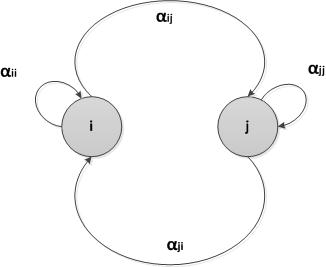
\includegraphics[height=0.28\textheight]{stateTrans.jpg}}
\caption{State Transition Probability between two sites $S_i$ and $S_j$}
\label{stateTrans}
\end{figure}

We introduce the notion of \emph{average function estimate} in the network $\vec{J_i^t} = \sum_i \frac{J_i^t}{k}$ which allocates equal weight to all the local function estimates and serves as a baseline against which individual sites $S_i$'s can compare their performance. Philosophically, this also implies that each local site should at least try to attain as much information as required to converge to the average function estimate. Since $\sum_i{\alpha_{ij}}=1$, this estimate is invariant. 

The $A$ matrix has interesting properties which allow us to show that convergence to $\vec{J_i^t}$ occurs. One such property is the Perron-Frobenius theory of irreducible non-negative matrices. We state the theorem here for continuity.

\begin{thm} \textbf{Perron-Frobenius \cite{Varga_62}}
Let $A$ be a positive, irreducible matrix such that the rows sum to 1. Then the following are true:
\begin{enumerate}
\item The eigenvalues of $A$ of unit magnitude are the $k$-th roots of unity for some $k$ and are all simple.
\item The eigenvalues of $A$ of unit magnitude are the $k$-th roots of unity if and only if $A$ is similar under a permutation to a $k$ cyclic matrix
\item all eigenvalues of $A$ are bounded by 1.
\end{enumerate}
\end{thm}

Since the eigenvalues of $A$ are bounded by 1, it can be shown that $J_i^t$ converges to the average function estimate $\vec{J_i^t}$ if and only if -1 is not an eigen value \cite{Varga_62}. Let $\lambda_n \le \lambda_{n-1} \le \cdots \le \lambda_2 < \lambda_1 =1$ be the eigenvalues of $A$ with $\lambda_1 = 1$. Also assume that $\gamma (A) = \text{max}_{i>1} |\lambda_i|$. It can be shown that $\parallel J_i^{t+1} - \vec{J}_i^{t} \parallel^2 \le \gamma^2 \parallel J_i^{t} - \vec{J}_i^{t} \parallel$. If $\gamma=1$, then system fails to converge \cite{Varga_62}, \cite{Cybenko_89}. \\
 
 
\noindent \textbf{Local Stochastic Gradient update} is done as follows: $W_i^{t+1} = W_i^t - \eta_i^t s_i^t$ where $s_i^t=\frac{\partial L_i^t}{\partial W_i^t}$ is the estimated gradient, $W_i^t$ is the weight vector and $\eta_i^t$ is the learning rate at node $i$ at time t. 
%It must also be noted that if $\eta_l^t$ be such that for positive constants $A_1, A_2$, $\frac{A_1}{t} \le \eta_l^t \le \frac{A_2}{t}, \forall t$, the learning rate requires only a local clock and runs in the same time scale as the global clock \cite{Tsitsiklis_86}. 
Let $s_i^t=\frac{\partial J_i^t}{\partial W_i^t} + \mathcal{W}_i^t$, where $\mathcal{W}_i^t$ is unit variance white noise independent for each site $S_i$. Then, it can be easily seen that $E[\parallel \mathcal{W}_i^t \parallel^2 |W_i^t] \le M (\parallel \nabla J_i^t \parallel^2)$, for some constant $M$. \\

%There is a large class of stochastic optimization algorithms where the \emph{expected} direction of update conditioned on the past history of the algorithm is a descent direction with respect to the cost function $J$ and these algorithms are called \emph{pseudo-gradient} algorithms \cite{Poljak_73}. In the following section we present convergence results for the pseudo-gradient distributed feature selection algorithm.


\noindent{\textbf{An empirical example:}} Consider the train spotting example introduced in Section~\ref{sec:example}. Assume that the $500$ randomly generated features\footnote{The Aleph software \texttt{http://www.cs.ox.ac.uk/activities/machlearn/Aleph/aleph.html} was used to generate the features.} are partitioned amongst two sites, such that each contains 250 features. A distributed computing environment is simulated using the peersim simulator\footnote{http://peersim.sourceforge.net/}. The distributed feature selection algorithm was run for a fixed number of iterations varying the learning rate of the algorithm. Figures~\ref{s0} and \ref{s1} show how the norm of the loss function varies with the number of iterations at each site eventually leading to convergence. 
%Careful examination of the weight vector at each site also reveals that there are positive weights for some of the features identified from domain knowledge thereby verifying that the algorithm.
\begin{figure}[h]
\centerline
{
%\subfigure[All boroughs, SVM confidence margin]
\subfigure[Site 1]
{%\includegraphics[width=2\columnwidth]{scoresc-regions.pdf}
%\includegraphics[width=\columnwidth]{scoreall-new.pdf}
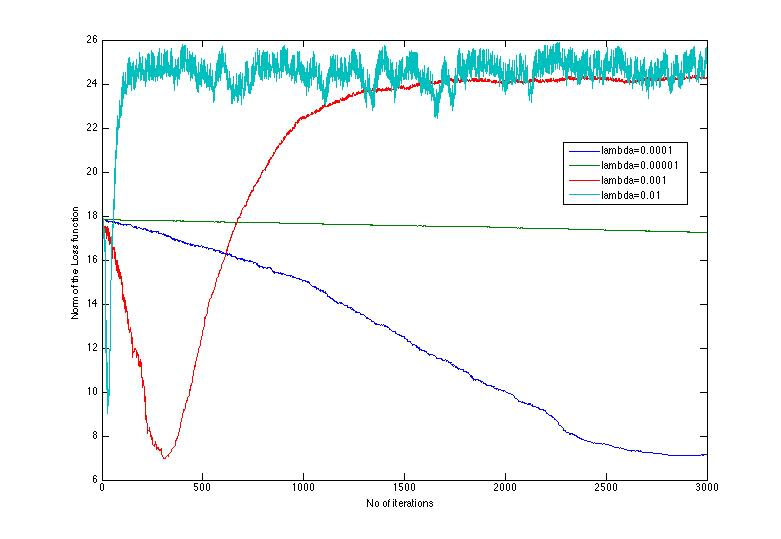
\includegraphics[width=0.55\textwidth,height=0.32\textheight]{Node_0.jpg}
  \label{s0}}\\
%\subfigure[Manhattan]
\subfigure[Site 2]
{%\includegraphics[width=\columnwidth]{scorescM.pdf}
%\includegraphics[width=\columnwidth]{scoremanhattan-new.pdf}  
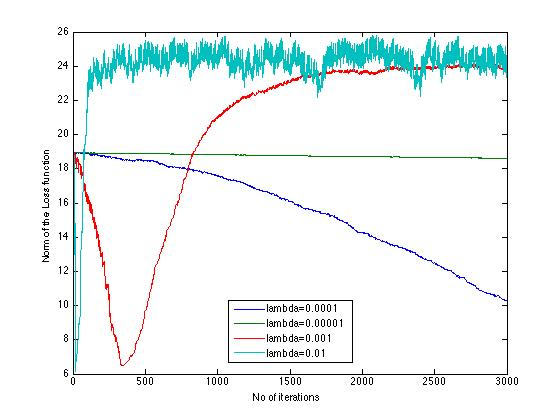
\includegraphics[width=0.55\textwidth,height=0.32\textheight]{Node_1.jpg}
\label{s1}}
}
\end{figure}

\subsection{Convergence}
\label{sec:algterm}
The proof of convergence of the algorithm has several sub-parts: (1) In the distributed setting, the process of information exchange between $k$ sites can be modeled as a non-stationary Markov chain. A non-stationary Markov chain is weakly ergodic if the dependence on the state distribution vanishes as time tends to infinity. Thus convergence of information exchange between sites needs to be established. This follows from the idea introduced by Tsitsiklis et al. \cite{Tsitsiklis_86}. It is based on proving convergence of a sequence of products of stochastic matrices (the $A$ matrix in our formulation) and the conclusions follow from well-known results on weak ergodicity of non-stationary Markov chains. (2) In a given iteration of the optimization, one needs to establish how good the approximated distributed optimization is compared to its ``ideal" central counterpart. This follows from the rich theory of approximate convex functions. 
We present an illustrative example and the basic notations and assumptions which eventually lead to the proof of convergence. (3) The number of iterations $T$ the algorithm requires to finally attain convergence in the distributed setting.

\noindent \textbf{An Example: } Consider two sites $S_1$ and $S_2$ with features $x_1, x_2$ and $x_3, x_4$ respectively. Site $S_1$ locally computes $J_{i}=[x_1 x_2][w_1 w_2]^T$ and Site $S_2$ computes $J_{j}=[x_3 x_4][w_3 w_4]^T$. Site $S_2$ sends $\alpha_{ji}J_{j}$ to $S_1$ and $S_1$ sends $\alpha_{ij}J_i$ to $S_2$. The local function estimates are updated to $J_i^{t+1}=\alpha_{ii}J_i + \alpha_{ji}J_{j}$ and $J_j^{t+1}=\alpha_{jj}J_j + \alpha_{ij}J_i$. Both $J_i$ and $J_j$ are convex functions \cite{Boyd_04} and $J_j^{t+1}$ and $J_i^{t+1}$ are simply perturbations of convex functions by bounded functions. This observation allows us to use the rich theory of Approximately Convex Functions (\cite{Hyers_52},\cite{Pales_02}) to show that the proposed algorithm will eventually converge.

\begin{defn}
\label{defn:1}
\textbf{Perturbation of Convex Functions by Bounded Functions (\cite{Pales_02}) : }Let $\delta \ge 0$ and $J: R^m \rightarrow R$ be of the form $J = g+h$, where $g:R^m \rightarrow R$, is convex and $\parallel h \parallel \le \delta$ i.e. $|h(x)| \le \delta, \forall x \in m$. Then, for all $x, y \in m$ and $t \in [0,1]$, 
$ f(tx + (1-t)y) = t f(x) + (1-t)f(y) + 2 \delta.$ More generally, $x_1, x_2 \cdots, x_n \in R^m$ and $t_1, \cdots ,t_n \in [0,1]$ with $t_1+ \cdots + t_n =1$, $f(t_1 x_1+ \cdots + t_n x_n) \le t_1 f(x_1) + \cdots + t_n f(x_n) + 2 \delta.$
\end{defn}

\begin{defn}
\label{defn:2}
\textbf{$\delta$-convex function: } Let $\delta \ge 0.$ Then a function $J: R^m \rightarrow R$ is called $\delta$-convex if $f(tx + (1-t)y) \le tf(x) + (1-t)f(y) + \delta, (x , y \in R^m, t \in [0,1])$
\end{defn}

\begin{thm}
\textbf{(Hyers and Ulam \cite{Hyers_52})} Let $J(x)$ be $\delta$-convex on the open convex set $G \subset R^m$ and $B$ be any closed bounded convex subset of $G$. Then, there exists a convex function $\phi(x)$ on $B$ such that $|\phi(x) - f(x)| \le k_m \delta$ where $k_m$ is a positive constant that depends only on the dimensionality $m$ and $k_m = \frac{m^2+3 m}{4m + 4}$.
\end{thm}
\noindent The above theorem can also be interpreted as follows: Assume that $J: R^m \rightarrow R$ is $\delta$-convex and is of the form $J=g+h$, where $g: R^{m} \rightarrow R, $ is a convex function and $h: R^{m} \rightarrow R,$ is a bounded function such that $\parallel h \parallel \le k_m \delta$ where $k_m$ depends only on the dimensionality $m$ as illustrated above.

Note that $f_g$ is defined over $\mathbb{R}^m$ while $f_i$ is applied on a subset of $\mathbb{R}^m$. Application of Hyers and Ulam theorem above, to each site $S_i$ clearly shows that $|f_i - f_g| \le k_m \delta$. This helps to characterize how good the local approximation is at each site when compared to the hypothetical centralized algorithm. 
% The weight vector at each site is $W_1^{t+1} = W_1^t - \eta_1^t s_1^t$ and $W_2^{t+1} = W_2^t - \eta_2^t s_2^t$. Now, $\frac{\partial J_1}{\partial W_1} = -X_1 (y_1 - J(X_1))$. After obtaining the update from site $S_2$, the estimated value of the function $J(X_1)$ is altered while the randomly chosen instance $X_1$ from Site $S_1$ and the true labels $y_1$ still remain the same. Let $\hat{J_1}$ be an approximation of $J_1$ being evaluated at $S_1$. $\parallel \frac{\partial J_1}{\partial W_1} - \frac{\partial \hat{J_1}}{\partial W_1} \parallel = \parallel X_1 (y_1 - J_i^{t+1}(X_1))-X_1 (y_1 - J_i^t(X_1) \parallel = \parallel X_1 (J_i^t(X_1) - J_i^{t+1}(X_1))\parallel= \parallel X_1 (J_i - \alpha_{ii}J_i - \alpha_{ji}J_{j} )\parallel$.

%\noindent \emph{Assumption 1: } $J$ is continuously differentiable and its derivative satisfies the Lipschitz condition 
%\begin{asm}
%$J$ is continuously differentiable and its derivative satisfies the Lipschitz condition $\parallel \nabla J(W) - \nabla J(W')\parallel \le B_0 \parallel W - W' \parallel, \forall W, W' \in R^m$ where $B_0$ is a nonnegative constant. 

%\label{asm:1}
%\end{asm}
% 
%\begin{asm}
%Let $W_i^\tau = \{W_i^0, W_i^1, \cdots W_i^t\}$ represent the sequence of the weight vectors from the initialization of the algorithm to time $t$ at site $S_i$. The updates $s_i^t$ at each processor satisfy $E[\frac{\partial J_i^t}{\partial W_i^t} \times s_i^t | \text{ } W_i^\tau ] \le 0$
%\end{asm} 
%\noindent Thus, each site's update is in a descent direction when conditioned on the past history of the algorithm. 

%\begin{asm}
%For some $B_1 \ge 0, \text{ } E[\parallel s_i^t  \parallel^2] \le -B_1 \text{ } E [\frac{\partial J_i^t}{\partial W_i^t} \times s_i^t] $
%\end{asm}

%\noindent Let $B^t = \sum_{i=1}^{k} \parallel s_i^t \parallel$. Then $(B^t)^2 \le k \times \sum_{i=1}^{k} \parallel s_i^t \parallel^2$.

\noindent \textbf{Termination criteria: } The distributed algorithm is run until $T$ iterations. The usual practice with stochastic gradient descent algorithms is to run them until the loss at each site is within a certain user-defined threshold. We follow the same principle here, but note that for the distributed algorithm, each site runs stochastic gradient descent locally and independently of any other site. This implies that the same example may not be chosen at each site and this affects the termination criteria.

%\subsection{Correctness}
%\label{sec:algcorrect}
\noindent \textbf{How many iterations are required for convergence?} Parameter updates performed on the cost function $J_k^t(W^{t}_k)$\footnote{Note that the cost function is explicitly parameterized by $W$ to indicate that $J_k^t$ depends on $W$. This is a slightly different notation than what we                                    used in Section~\ref{sec:probdesc}.} at site $S_k$ are based on the sample $X_p =(X_p^1, \cdots, X_p^{m_k}), p \in \{1, \cdots, n\}$ chosen from $M_k$. $L_k^t(W^{t}_k)$ can be expressed as a very large sum of terms i.e. $L_k^t(W^{t}_k)=\frac{1}{n} \sum_{p=1}^{n} L^{t}_k(X_p,W^{t}_k)$. The parameter update using Stochastic Gradient Descent (SGD) can be written as
\begin{equation}
\label{localOpt1}
W^{t+1}_k = W^{t}_k - \frac{1}{t} \phi_t \frac{\partial L^{t}_k }{\partial W^{t}_k}(X_p, W^{t}_k)
\end{equation}
where $\phi_t$ is an appropriately chosen positive semi-definite matrix. 

Simple batch algorithms where the gradient is estimated over \emph{all} the training examples, converge linearly to the optimum $W^{*}_k$ of the empirical cost. In contrast, when using an SGD algorithm, it can be shown that under mild assumptions, the optimization converges to a local minimum of the cost \cite{bottou-98x,Benveniste_90,Bertsekas_97}. It appears that SGD-based algorithms converge to the general area of the optimum as fast as batch algorithms, but tend to wobble around in that region due to the noisy estimation of the gradient. It has been shown that $\textbf{E}(W^{t}_k - W^{*}_k)$ converges like $\frac{1}{t}$ at best \cite{Bottou_05}. 

The above observation can also be explained as follows: since the measurement of the gradient is noisy, we do not have access to $L_k^t(W^{t}_k)$ but to a noisy variant of it $\frac{\partial L_k^t }{\partial W_k^t}(X_p, W_k^t) + \delta_k^t$ where $\delta_k^t$ is a random variable representing the noise. If we used the gradient algorithm as if no noise were present, Equation~\ref{localOpt1} can be re-written as:
\begin{equation}
\label{localOpt2}
W^{t+1}_k = W^{t}_k - \frac{1}{t} \phi_t (\frac{\partial L^{t}_k }{\partial W^{t}_k}(X_p, W^{t}_k) + \delta_k^t)
\end{equation}
Equation~\ref{localOpt2} does not converge to a minimum of $L^{t}_k$ and what may happen at best is that $W^{t}_k $ converges to a local minima and moves randomly about $W^{*}_k $. The mean square distance of $W^{t}_k $ from $W^{*}_k$ increases with variance of $W^{t}_k$ and can be made small only if $\eta_k^t$ is chosen small. If $\eta_k^t$ is chosen to be very small it can take a very large number of steps to reach a neighborhood of a local minima. To strike a balance, $\eta_k^t$ is usually set to $\frac{1}{t}$ which allows a rapid approach to the vicinity of the $W^{*}_k$ and then decreased to zero, so that the variance of $W^{t}_k$ also reduces. Some typical conditions set on the step size are: $\sum_{t=1}^{\infty}\eta_k^t=\infty$ and $\sum_{t=1}^{\infty}(\eta_k^t)^2 <\infty$. 
%Let $V(t)$ be the variance of $W^{t}_k$. If $\delta_k^t$ is independent of $W^{t}_k$ and has a variance $\sigma_k^2$ then the variance of $W^{t+1}_k$ is given by

In our distributed setting, let $W^{*}_k$ be the local optimum of the cost $J_k^t(W)$ and $W^{*}_g$ be the global optimum of the cost $J_g^t(W)$ involving all the attributes over the network. We would like to know how fast $W_k$ converges to $W^{*}_g$ instead of $W^{*}_k$. This implies we need to study the effect of perturbation of $J_k^t(W)$ on convergence of the algorithm to the global solution.

\begin{figure}[h]
\centerline{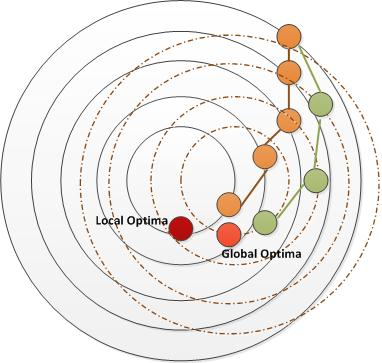
\includegraphics[width=0.68\textwidth]{contours.jpg}}
\caption{Contour of the local and global optimization at a site. The brown concentric circles indicate the perturbation of the local cost to learn the global cost. The path traced by the yellow ochre colored circles indicate a possible optimization path if only the local cost were considered. The green colored circles show the path if the global cost were to be optimized. }
\label{convergence}
\end{figure}

Bottou and Le Cun~(\cite{Bottou_05},\cite{lecun-98a}) show that 
\begin{equation}
W^{*}_t = W^{*}_{t-1} - \frac{1}{t} \hat{H}_n^{-1} \frac{\partial J}{\partial W} (X_p,W^{*}_{t-1} ) + \mathcal{O}_u(\frac{1}{n^2})
\end{equation}
where empirical Hessian are defined as $\hat{H}_n = \frac{1}{n} \sum_{i=1}^{n} \frac{\partial^{2}}{\partial \theta \partial \theta} L(X_p, W^{*}_{t-1}) $

%
%\subsection{Parameters of the algorithm}

%\begin{itemize}
%\item The number of nodes in the network
%\item The degree distribution of the nodes
%\item The choice of B matrix and hence $\alpha$ among nodes
%\item The splitting of data on the nodes -- relax the hard splits and allow multiple splits and over-laps
%\item The learning parameter of the algorithm 
%\end{itemize}
%\subsection{An Algorithm Using Distributed Randomized Local Search for Feature Construction}

%\begin{algorithm}[H]
%\SetKwData{Left}{left}\SetKwData{This}{this}\SetKwData{Up}{up}
%\SetKwFunction{Union}{Union}\SetKwFunction{FindCompress}{FindCompress}
%\SetKwInOut{Input}{input}\SetKwInOut{Output}{output}

%%\Input{$n \times m_i$ matrix at each site $S_i$; \\
%%	   $G(V, E)$ which encapsulates the underlying communication framework; \\
%%	   $T: $ no of iterations} 
%\KwIn{ Each site $S_i$ has (i) background knowledge $B$, (ii) a set of examples $E$ vertically partitioned, (iii) a set of class labels $\mathcal{Y} = \{1, 2, \cdots, c \}$, (iv) sample size $n, (1 \le n)$, (v) the minimal support for acceptable clauses $s, (1 \le s)$, (vi) the minimal precision for acceptable clauses $p, (0 < p \le 1)$, (vii) a language $\mathcal{L}$ specifying constraints on acceptable clauses that can be considered in the search for any feature, (viii) the number of random restarts $R$, (ix) the number of local moves $M$.     }
%\KwOut{Each site $S_i$ has $W_i \approx W_g[1: m_i]$. The acceptable features are those with highest weights in $W_i$ }
%%\Output{Each site $S_i$ has $W_i \approx W_g[1: m_i]$ }
%\BlankLine
%\nl $F_i=\{\}$ \;
%\nl \For {i=1 to $R$} 
%	{
%	currentFeatures= sample of acceptable features given $B, E, \mathcal{Y}, n, s, p, \mathcal{L} $
%	}
% %
% %\KwData{$n \times m_i$ matrix at each site $S_i$; Graph $G(V, E)$ which encapsulates the underlying communication framework; $T: $ no of iterations}
% %\KwResult{Each site $S_i$ has $W_i \approx W_g[1: m_i]$ }
% %initialization\;
%\For{i = 1 to T}
% {
%  Site $S_i$ computes $M_i W_i^T$ locally and estimates the loss function\;
%  Site $S_i$ gossips with its neighbors $S_j \in \{N_i\}$ and obtains $M_j W_j^T$ for each neighbor\;
%  Site $S_i$ locally updates its function estimate as $J_i^t = \alpha_{ii}(M_i W_i^T) + \alpha_{ji} (M_j W_j^T)$ \;
%  Update the local weight vectors using stochastic gradient descent as follows: $\frac{\partial J_i}{\partial W_i} = -M_i (y_i - f(x_i))$
% }
% 
%\caption{Distributed Feature Estimation}
%\label{alg:fs}
%\end{algorithm}


\section{Experimental Evaluation}
\label{sec:expt}

\subsection{Aims}
\label{sec:exptaims}
\subsection{Materials}
\label{sec:exptmat}

\subsection{Method}
\label{sec:exptmeth}

%\subsection{How fast is the algorithm compared to existing ones?}

%\subsection{How does the training time scale with number of training examples?}
%are there bottlenecks -- degradation of performance due to gossip?

%\subsection{How small does $\epsilon$ get?}

%\subsection{How good is the ranking of features?}

%\subsection{How good is the predictive performance of the algorithm?}
%\label{sec:exptresults}

\section{Results and Discussion}



\section{Conclusion}
\begin{acknowledgements}
This work began when Haimonti Dutta visited the Indraprastha Institute of Information Technology, Delhi in Spring 2013. She was also supported by National Science Foundation grant, IIS-0916186. The classification of literature on discriminative feature selection in ILP applications was first suggested by Ganesh Ramakrishnan.
\end{acknowledgements}

% BibTeX users please use one of
%\bibliographystyle{spbasic}      % basic style, author-year citations
\bibliographystyle{spmpsci}      % mathematics and physical sciences
%\bibliographystyle{spphys}       % APS-like style for physics
\bibliography{fs}   % name your BibTeX data base

% Non-BibTeX users please use
%\begin{thebibliography}{}
%
% and use \bibitem to create references. Consult the Instructions
% for authors for reference list style.
%
%\bibitem{RefJ}
% Format for Journal Reference
%Author, Article title, Journal, Volume, page numbers (year)
% Format for books
%\bibitem{RefB}
%Author, Book title, page numbers. Publisher, place (year)
% etc
%\end{thebibliography}

\end{document}
% end of file template.tex

